\chapter{نمودار‌های آموزش شبکه}\label{app:figs}
به عنوان نمونه، بعضی از مهم‌ترین نمودار‌های آموزش مدل‌های پیشنهادی ۱ و ۲ با دادگان \amazon{} در ذیل آمده است. لازم به ذکر است در تمامی نمودار‌ها، محور‌ افقی
\trans{تعداد دفعات دیدن کل داده‌ها}{Epoch}
است.
\begin{figure}[h]
	\centering
	\begin{subfigure}{0.3\textheight}
		\centering
		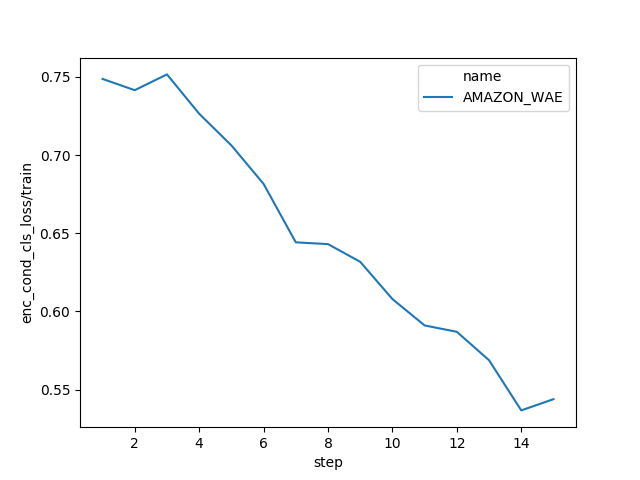
\includegraphics[width=1.\textwidth]{images/figs2/2020_01_15__11_37_34__enc_cond_cls_loss.png}
		\caption{}
		\label{fig:chap4:amazon_enc_cls}
	\end{subfigure}
	\begin{subfigure}{0.3\textheight}
		\centering
		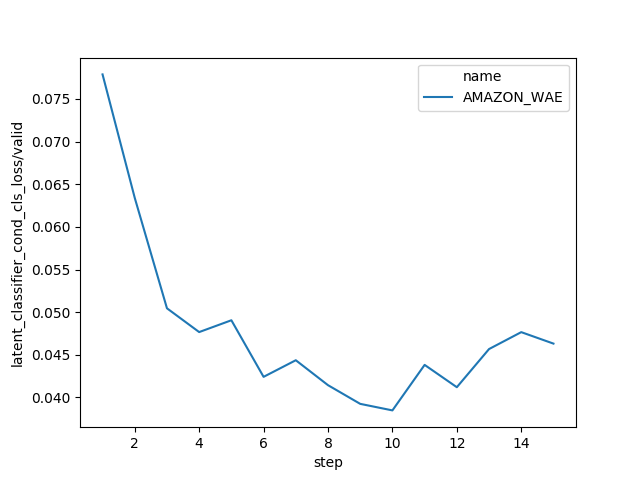
\includegraphics[width=1.\textwidth]{images/figs2/2020_01_15__11_37_34__latent_classifier_cond_cls_loss.png}
		\caption{}
		\label{fig:chap4:amazon_latent_cls}
	\end{subfigure}
	\begin{subfigure}{0.3\textheight}
		\centering
		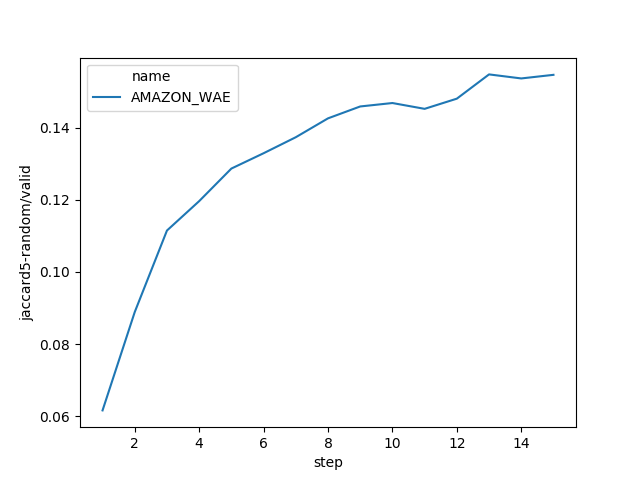
\includegraphics[width=1.\textwidth]{images/figs2/2020_01_15__11_37_34__jaccard5-random.png}
		\caption{}
		\label{fig:chap4:amazon_jaccard}
	\end{subfigure}
	\begin{subfigure}{0.3\textheight}
		\centering
		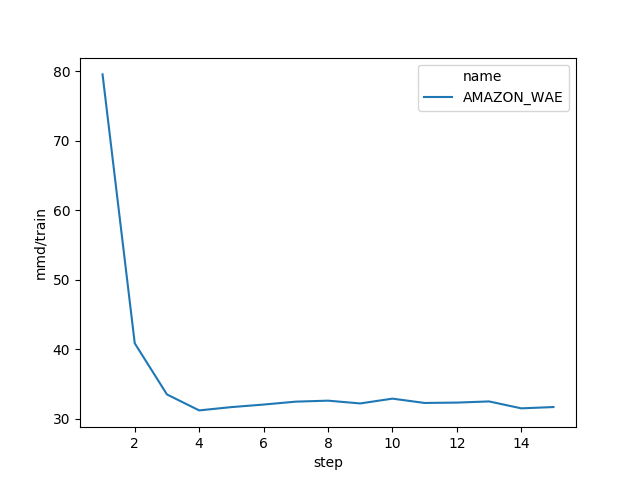
\includegraphics[width=1.\textwidth]{images/figs2/2020_01_15__11_37_33__mmd.png}
		\caption{}
		\label{fig:chap4:amazon_mmd}
	\end{subfigure}
	\begin{subfigure}{0.3\textheight}
		\centering
		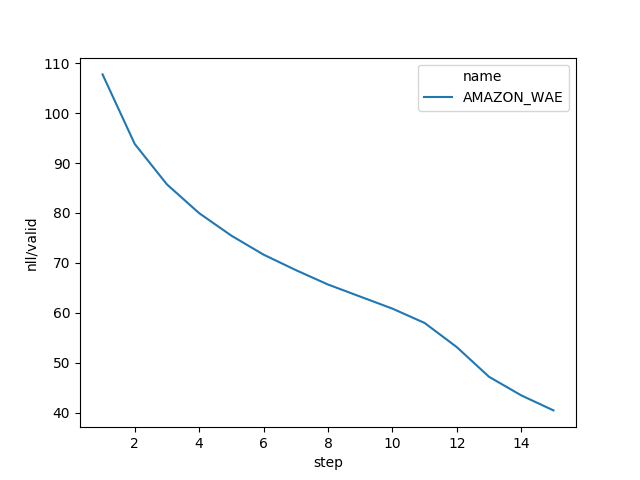
\includegraphics[width=1.\textwidth]{images/figs2/2020_01_15__11_37_34__nll.png}
		\caption{}
		\label{fig:chap4:amazon_nll}
	\end{subfigure}
	\caption
	[
		مدل پیشنهادی ۱.
		نمودار‌های آموزش \wae{} بر روی دادگان \amazon{}.
	]
	{
		مدل پیشنهادی ۱.
		نمودار‌های آموزش \wae{} بر روی دادگان \amazon{}.
		هزینه دسته‌بندی بردار‌های نهان تولید شده توسط \encoder{}
		(\subref{fig:chap4:amazon_enc_cls})؛
		هزینه دسته‌بندی \classifier{} در فضای نهان
		(\subref{fig:chap4:amazon_latent_cls})؛
		کیفیت و تنوع جملات تولیدی با توجه به معیار \jaccard{}
		(\subref{fig:chap4:amazon_jaccard})؛
		فاصله توزیع \marginal{} \encoder{} و \priordist{} با توجه به معیار \mmd{}
		(\subref{fig:chap4:amazon_mmd})؛
		خطای بازسازی جملات
		(\subref{fig:chap4:amazon_nll}).
	}
	\label{fig:chap4:amazon_cond}
\end{figure}


\begin{figure}[h]
	\centering
	\begin{subfigure}{0.3\textheight}
		\centering
		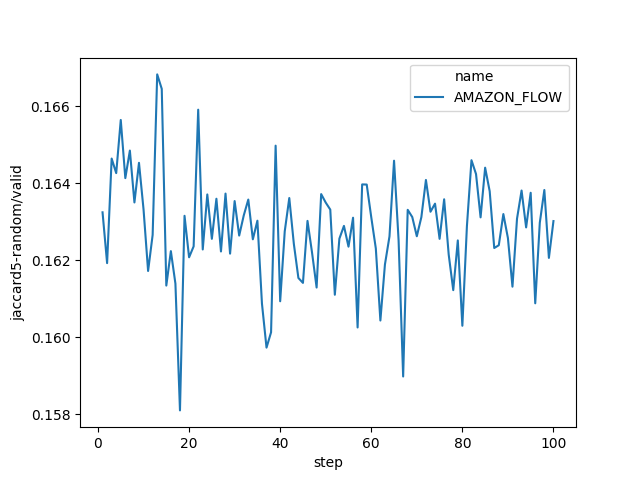
\includegraphics[width=1.\textwidth]{images/figs2/2020_01_15__11_41_02__jaccard5-random.png}
		\caption{}
		\label{fig:chap4:amazon_flow_jaccard}
	\end{subfigure}
	\begin{subfigure}{0.3\textheight}
		\centering
		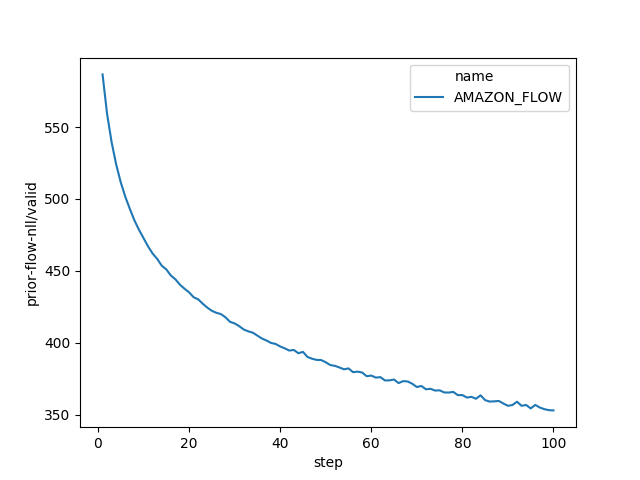
\includegraphics[width=1.\textwidth]{images/figs2/2020_01_15__11_41_01__prior-flow-nll.png}
		\caption{}
		\label{fig:chap4:amazon_flow_nll}
	\end{subfigure}
	\caption
	[
		مدل پیشنهادی ۱. نمودار‌های آموزش مولد شرطی بر روی دادگان \amazon{}.
	]
	{
		مدل پیشنهادی ۱. نمودار‌های آموزش مولد شرطی بر روی دادگان \amazon{}.
		کیفیت و تنوع جملات تولیدی تولید شده توسط مدل مولد شرطی با توجه به معیار \jaccard{}
		(\subref{fig:chap4:amazon_flow_jaccard})؛
		تابع هزینه آموزش مولد شرطی
		(\subref{fig:chap4:amazon_flow_nll}).
	}
	\label{fig:chap4:amazon_flow}
\end{figure}

\begin{figure}[h]
	\centering
	\begin{subfigure}{0.3\textheight}
		\centering
		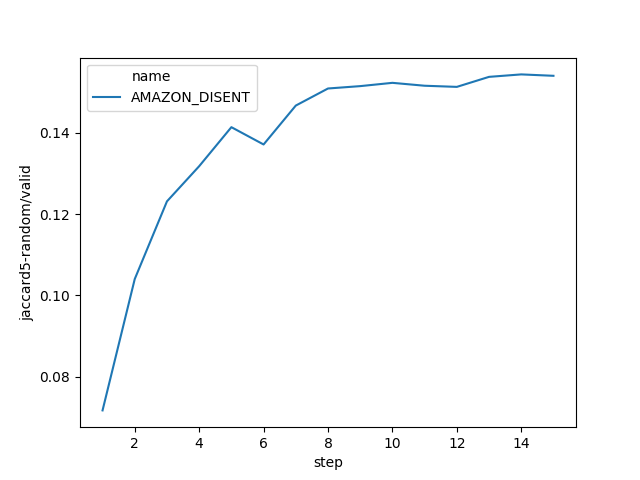
\includegraphics[width=1.\textwidth]{images/figs2/2020_01_15__11_42_11__jaccard5-random.png}
		\caption{}
		\label{fig:chap4:amazon_disent_jaccard}
	\end{subfigure}
	\begin{subfigure}{0.3\textheight}
		\centering
		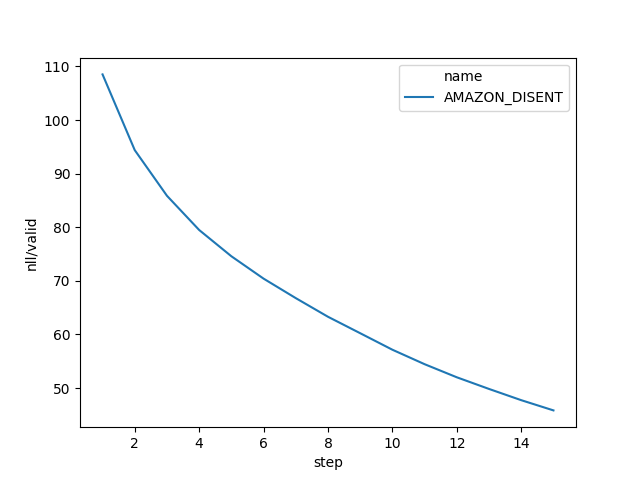
\includegraphics[width=1.\textwidth]{images/figs2/2020_01_15__11_42_11__nll.png}
		\caption{}
		\label{fig:chap4:amazon_disent_nll}
	\end{subfigure}
	\begin{subfigure}{0.3\textheight}
		\centering
		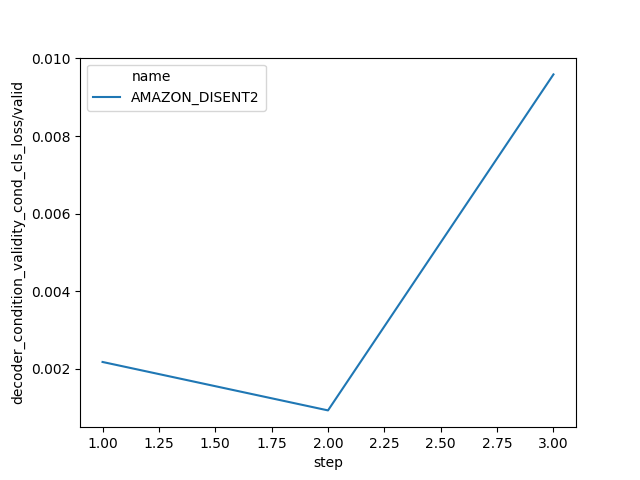
\includegraphics[width=1.\textwidth]{images/figs2/2020_01_15__12_10_34__decoder_condition_validity_cond_cls_loss.png}
		\caption{}
		\label{fig:chap4:amazon_disent_xcls}
	\end{subfigure}
	\begin{subfigure}{0.3\textheight}
		\centering
		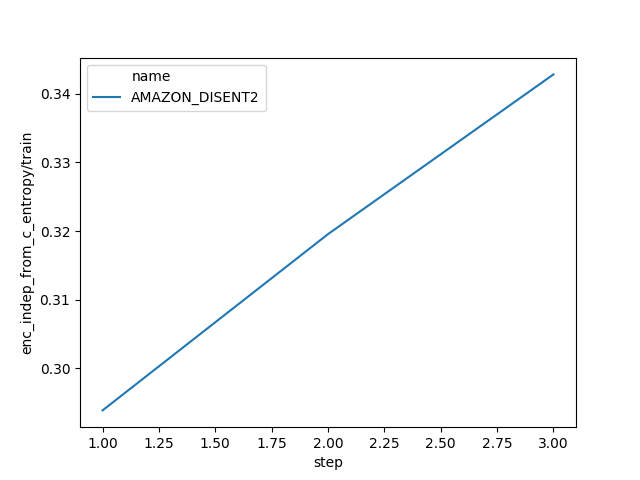
\includegraphics[width=1.\textwidth]{images/figs2/2020_01_15__11_44_04__enc_indep_from_c_entropy.png}
		\caption{}
		\label{fig:chap4:amazon_disent_indp}
	\end{subfigure}
	\begin{subfigure}{0.3\textheight}
		\centering
		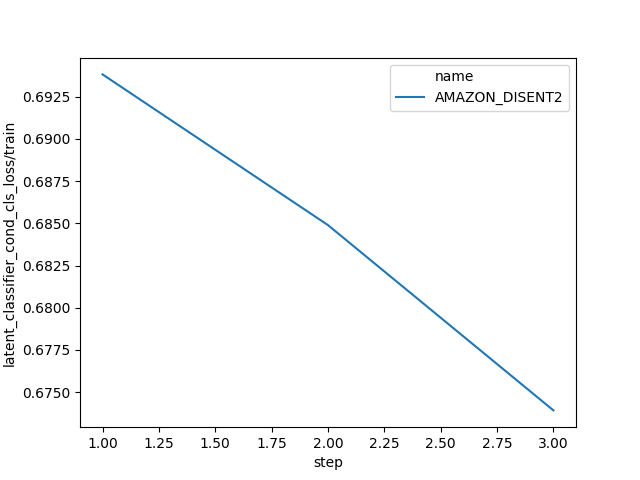
\includegraphics[width=1.\textwidth]{images/figs2/2020_01_15__11_44_04__latent_classifier_cond_cls_loss.png}
		\caption{}
		\label{fig:chap4:amazon_disent_latent_cls}
	\end{subfigure}
	\caption
    [
    		مدل پیشنهادی ۲. نمودار‌های آموزش مدل بر روی دادگان \amazon{}.
    ]
    {
		مدل پیشنهادی ۲. نمودار‌های آموزش مدل بر روی دادگان \amazon{}.
		کیفیت و تنوع جملات تولیدی تولید شده توسط \decoder{} شرطی با توجه به معیار \jaccard{}
		(\subref{fig:chap4:amazon_disent_jaccard})؛
		خطای بازسازی
		(\subref{fig:chap4:amazon_disent_nll})؛
		تابع هزینه دسته‌بندی جملات
		(\subref{fig:chap4:amazon_disent_xcls})؛
		استقلال فضای نهان از شرط (آنتروپی \classifier{})
		(\subref{fig:chap4:amazon_disent_indp})؛
		استقلال فضای نهان از شرط (هزینه دسته‌بندی \classifier{} در فضای نهان)
		(\subref{fig:chap4:amazon_disent_latent_cls}).
	}
	\label{fig:chap4:amazon_disent}
\end{figure}
